%%% template.tex
%%%
%%% This LaTeX source document can be used as the basis for your technical
%%% paper or abstract. Regardless of the length of your document, the commands
%%% are all the same.
%%% 
%%% The "\documentclass" command is the first command in your file. If you want to 
%%% prepare a version of your article with line numbers - a "review" version - 
%%% include the "review" parameter:
%%%    \documentclass[review]{acmsiggraph}
%%%

\documentclass{acmsiggraph}
\usepackage{listings,verbatim,csquotes}

%%% Title of your article or abstract.

\title{Combination of Ray and Wave Optics For Vision Correcting Display}

\author{
	Charles Ding\\
	\text{M.S. in EECS, University of California, Berkeley}
	\and
	Luxin Yang\\
	\text{M.S. in EECS, University of California, Berkeley}
}
\pdfauthor{Charles Ding, Luxin Yang}

%%% Used by the ``review'' variation; the online ID will be printed on 
%%% every page of the content.

\TOGonlineid{45678}

% User-generated keywords.

\keywords{ray optics, wave optics, vision}

%%% The next five lines define the rights management block on the first page.
%%% Replace them with the LaTeX commands provided when the form has been completed.

\CopyrightYear{2016}
\setcopyright{acmcopyright}
\conferenceinfo{CS294-127: Computational Imaging}{December, 9, and 2016} 
\isbn{445-6-95-609353-5}\acmPrice{\$0.00}
\doi{http://doi.acm.org/vision/correcting/display}

%%% Start of the document.

\begin{document}
\lstset{language=C++, breaklines=true, basicstyle=\ttfamily\small}   

%%% This is the ``teaser'' command, which puts an figure, centered, below 
%%% the title and author information, and above the body of the content.

\teaser{
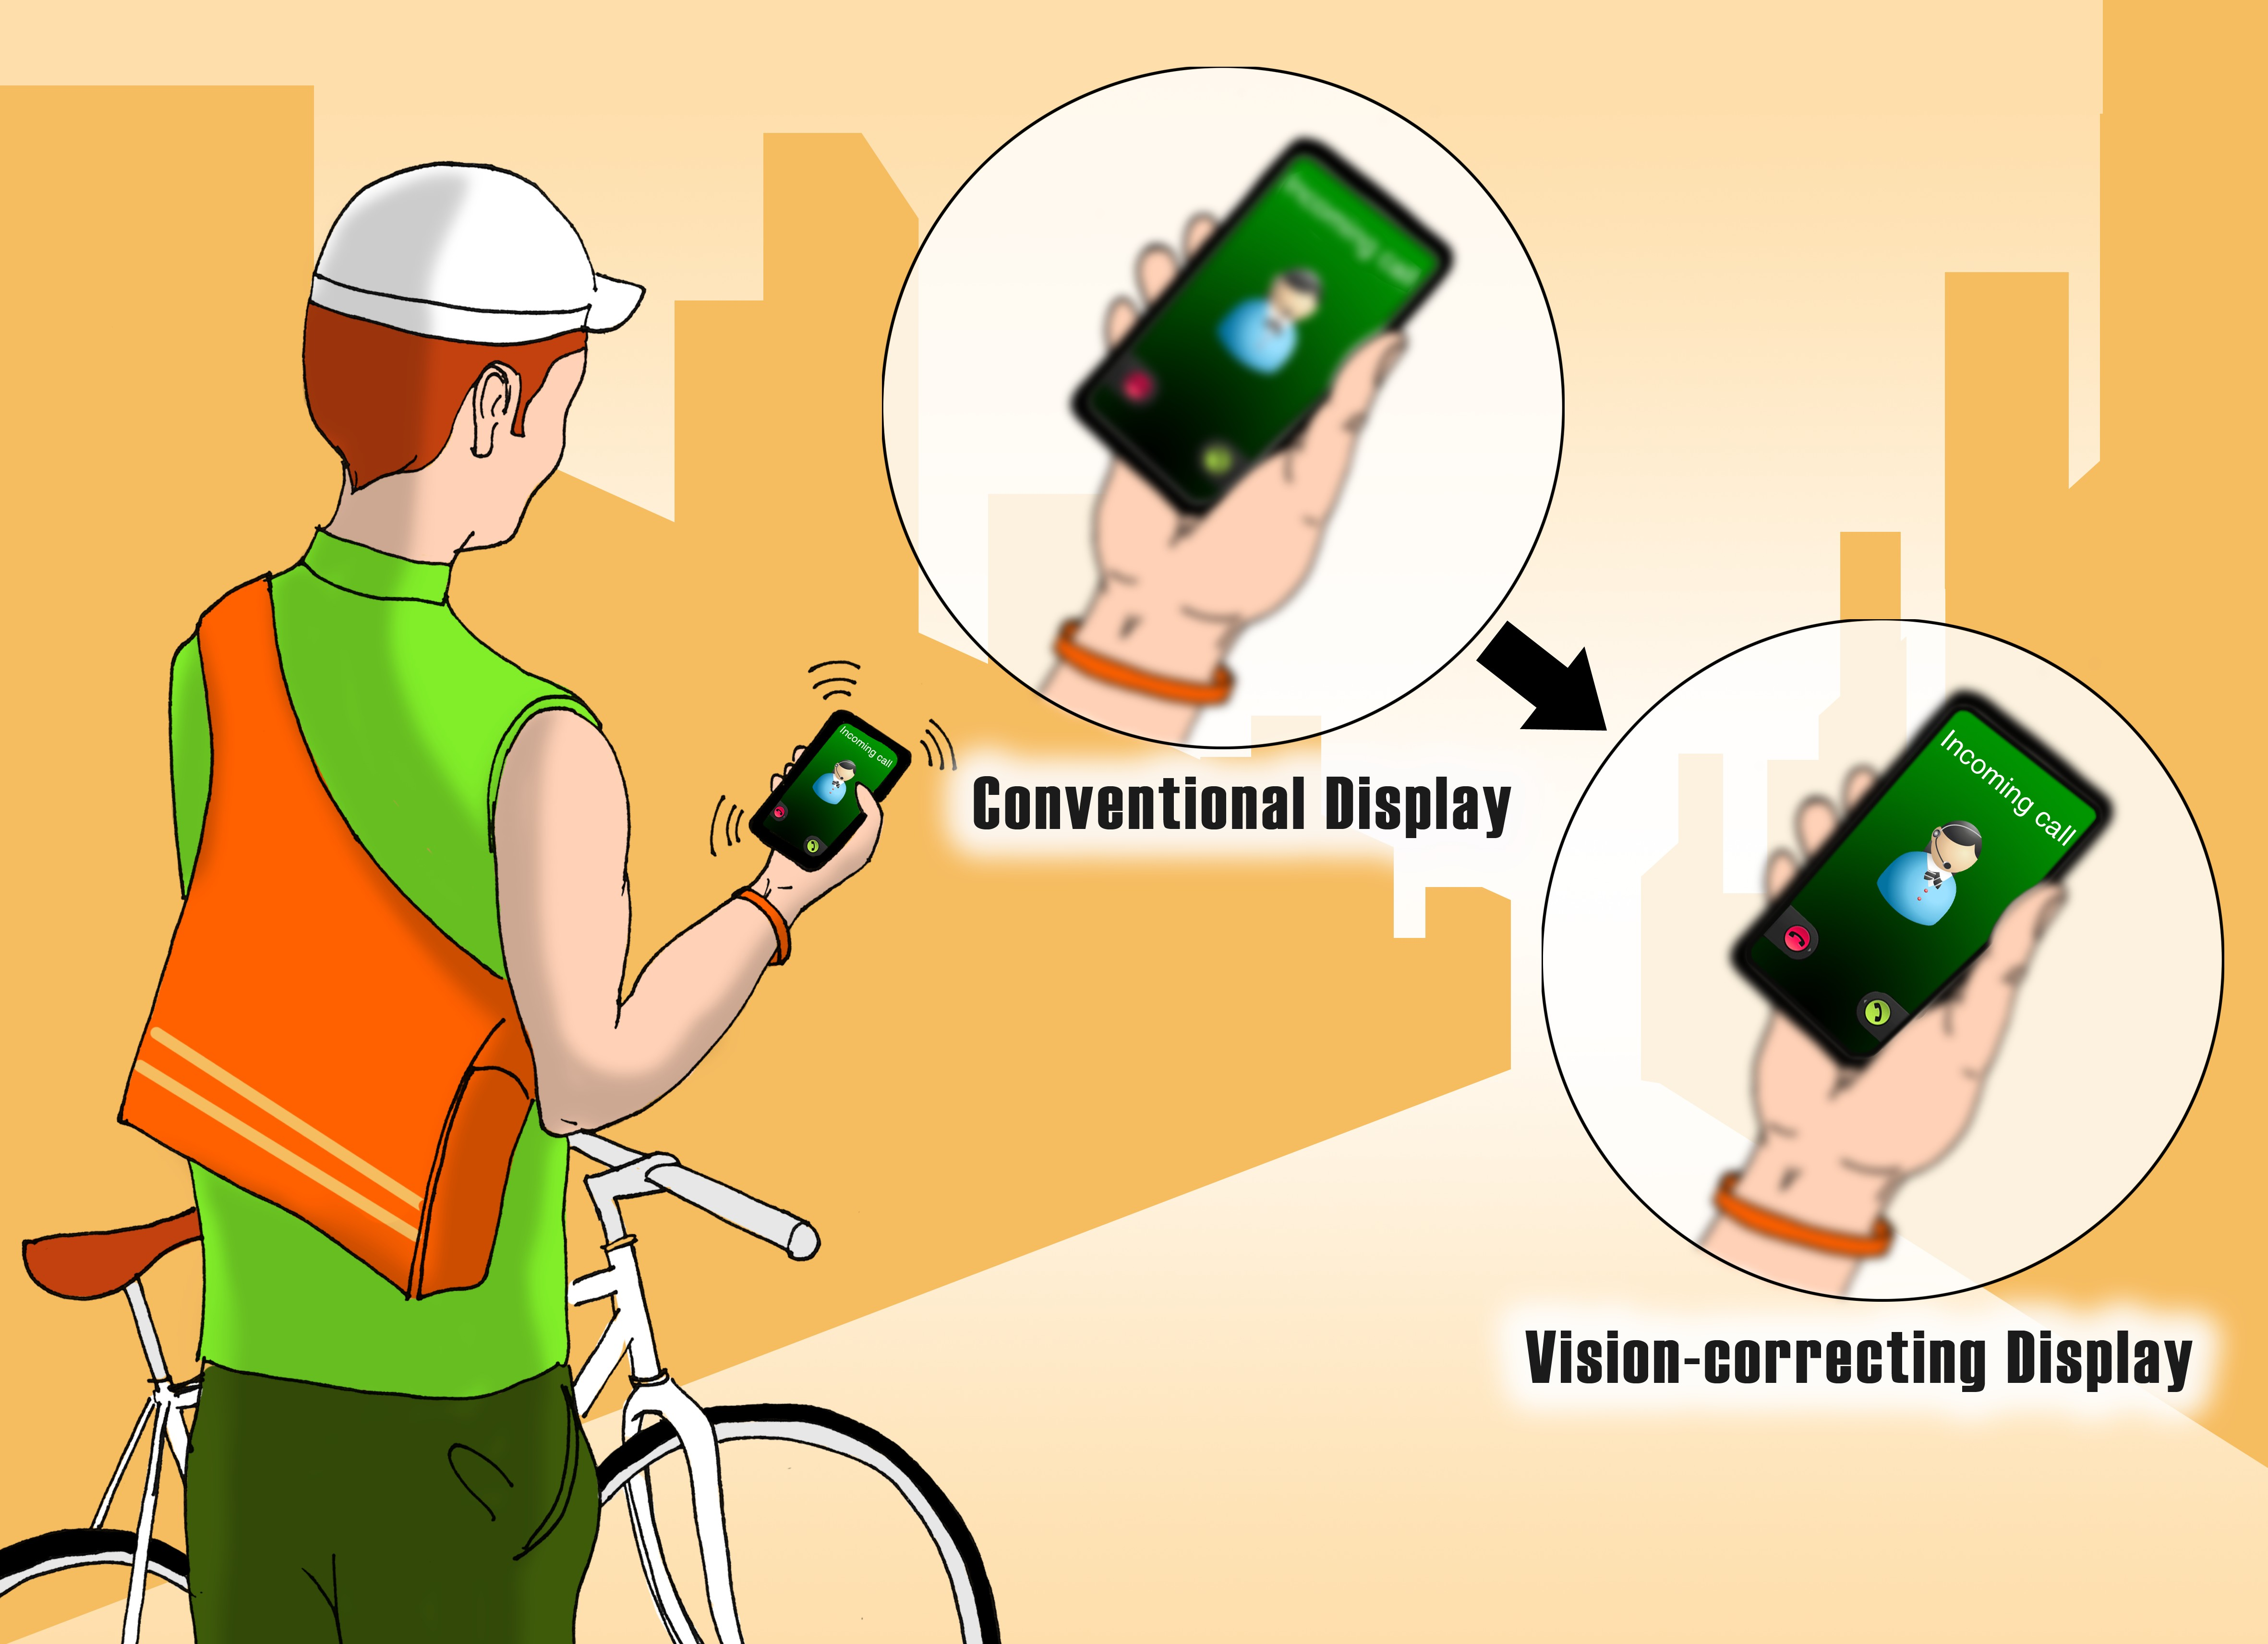
\includegraphics[height=1.5in]{phone}
  \caption{[Huang et al. 2014]: Application Scenario of Vision-Correcting Display}
}

\maketitle

\begin{abstract}

Human vision problems such as near-sightedness and far-sightedness are a result of optical aberrations in the human eye. The common method of treating eye aberrations is wearing corrective lenses, such as glasses or contact lenses, or undergoing laser eye surgery. According to the Vision Council, roughly 75 percent of all adults in the United States require some form of vision correction [GlassesCrafter.com 2010]. The vision correcting display team under Professor Brian Barsky aims to develop a display using hardware and software that lets the user see a digital screen clearly without glasses or contact lenses. In addition, the team writes software simulations of the vision correcting display to evaluate the performance of the display for different eye aberrations and different digital devices. We present two different approaches to the software simulation, one using purely ray optics, and one combining wave and ray optics, and compare the results of both approaches with that of the physical experiment.

\end{abstract}

%
% The code below should be generated by the tool at
% http://dl.acm.org/ccs.cfm
% Please copy and paste the code instead of the example below. 
%
\begin{CCSXML}
<ccs2012>
<concept>
<concept_id>10010147.10010371.10010382</concept_id>
<concept_desc>Computing methodologies~Image manipulation</concept_desc>
<concept_significance>500</concept_significance>
</concept>
<concept>
<concept_id>10010147.10010371.10010382.10010236</concept_id>
<concept_desc>Computing methodologies~Computational photography</concept_desc>
<concept_significance>300</concept_significance>
</concept>
</ccs2012>
\end{CCSXML}

\ccsdesc[500]{Computing methodologies~Image manipulation}
\ccsdesc[300]{Computing methodologies~Computational photography}

%
% End generated code
%

% The next three commands are required, and insert the user-generated keywords, 
% The CCS concepts list, and the rights management text.
% Please make sure there is a blank line between each of these three commands.

\keywordlist

\conceptlist

\printcopyright

\section{Introduction}

\noindent 
Humans depend on their vision for every waking hour of the day. Out of the five main senses, vision is arguably the most important in acquring information about the surrounding environment. A person cannot walk in the streets, drive a car, or read if he or she cannot see. However, genetic inheritance, disease, and age will naturally lead to the loss of vision. Professor Brian A. Barsky has been focusing on this field for over a decade and introduces to the concept of the vision correcting display in his paper \textit{An Overview of Vision Realistic Rendering and Vision Correcting Displays} [2015]:

\begin{displayquote}
The concept of a vision correcting display involves digitally modifying the content of a display using measurements of the optical aberrations of the viewer's eye so that the display can be seen in sharp focus by the user without requiring the use of eyeglasses or contact lenses. Given the measurements of the optical aberrations of a users eye, a vision correcting display will present a transformed image that when viewed by this individual will appear sharp focus. Vision correction could be provided in some cases where spectacles are ineffective.
\end{displayquote}

\section{Vision Correcting Display}

The vision correcting display is composed of a hardware component, the pinhole mask display, and a software component, the prefiltering algorithm.

\subsection{Pinhole Mask Display}

The pinhole mask display is a light field display that is composed of a sheet of black film taped to a layer of acrylic 6 millimeters thick. The black film is composed of a 2D array of pinholes in the shape shown in Figure 2.

\begin{figure}[ht]
  \centering
  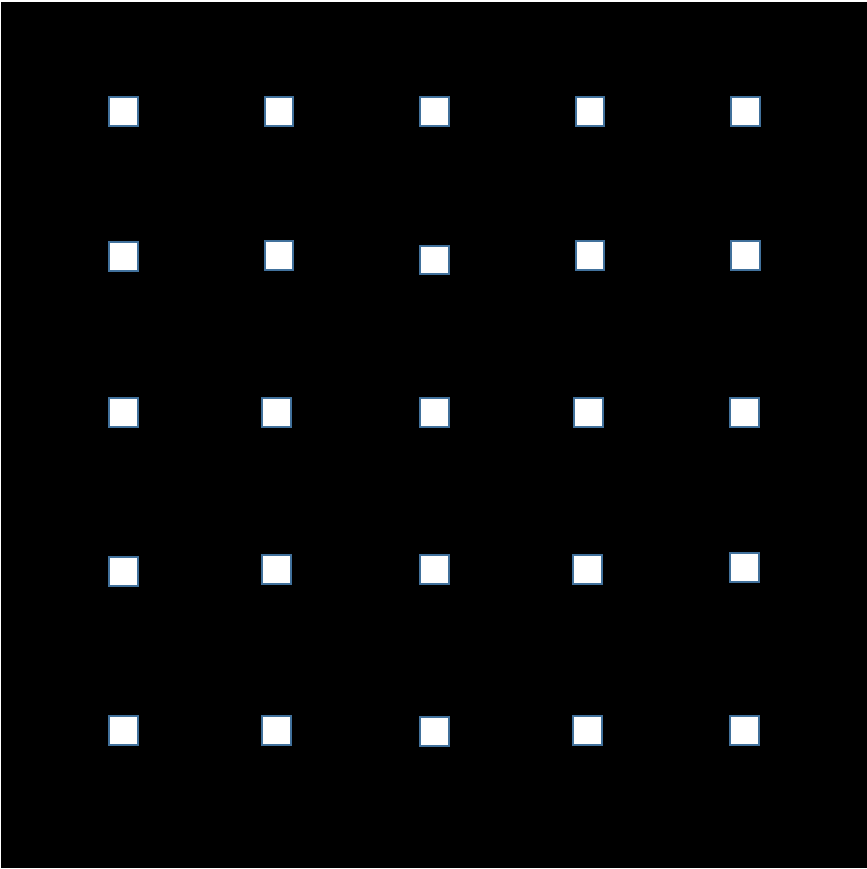
\includegraphics[width=1.5in]{Pinhole_Mask2}
  \caption{Area blocked and covered by pinhole.}
  \label{fig:ferrari}
\end{figure}

Previously, Huang et al. 2014 developed a similar light field display. However, Huang's display was a multilayer display, with a 2 millimeters screen protector placed on top of the pinhole film, which was on top of a 4 millimeter spacer, while we used a single layer display. Both Huang's display and our display had pinholes of size 75 micrometers that are 390 micrometers apart. Huang's display is used for the Apple iPod touch 4th generation display, which has a pixel pitch of 78 micrometers and resolution of $960 \times 640$ pixels, while our display is used for the iPhone 6, which has a resolution of $1334 \times 750$ pixels. Our pinhole mask has a greater depth (6 mm instead of 4 mm), and this increased depth allowed the outer pixels in the $5x5$ superpixel covered by the pinhole to become more visible. The light rays from the outer pixels travel at an angle through the pinhole mask and will miss the pupil if the angle was too large.

\begin{figure}[ht]
  \centering
  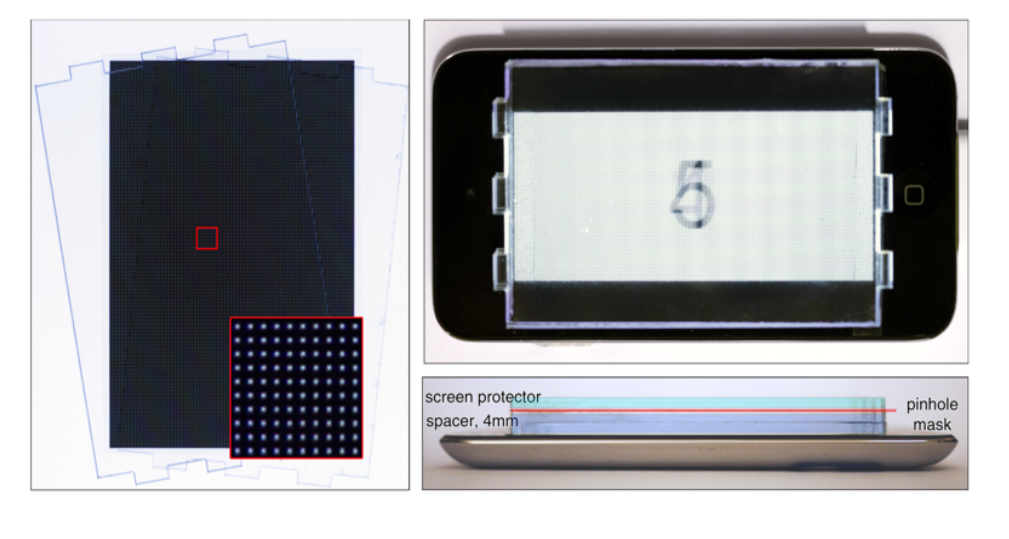
\includegraphics[width=3.0in]{Pinhole_Mask}
  \caption{[Huang et al. 2014]: Hardware prototype for light field construction.}
  \label{fig:ferrari}
\end{figure}

The goal of the pinhole mask is to focus the different light rays coming out of the screen, much like a pinhole camera or pinhole glasses. The display presents a 4D light field to the observer, which creates a 2D projection on the retina. Our goal is to make the 2D projection as close as possible to the original image. 

\subsection{Prefiltering Algorithm}

\begin{figure}[ht]
  \centering
  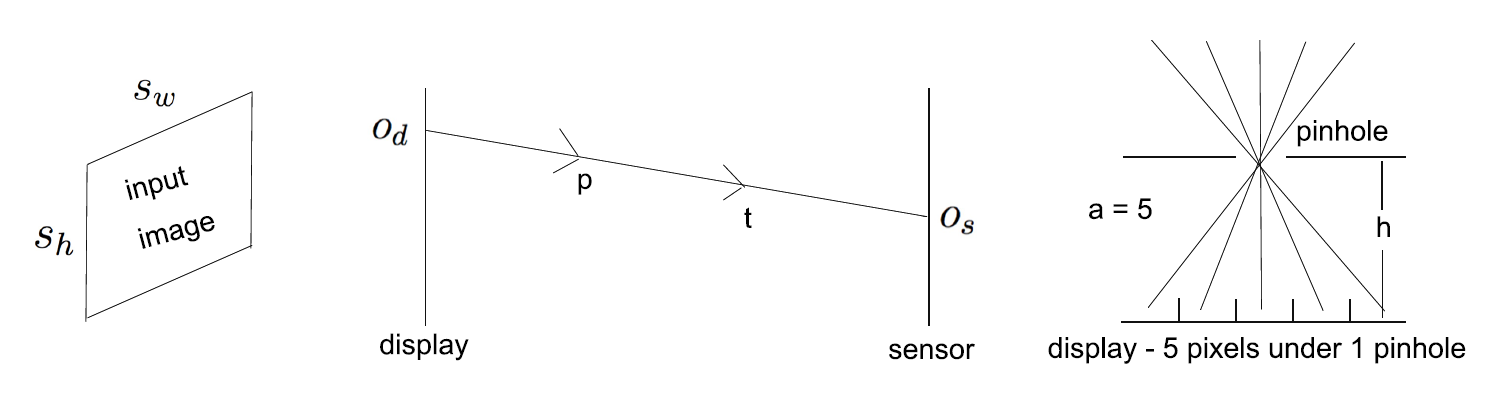
\includegraphics[width=3.0in]{Prefilter.png}
  \caption{The figure shows the setup for the prefiltering algorithm. (left) The input image has dimensions $s_w$ by $s_h$ pixels. (middle) $p$ and $t$ are points on the light ray. (right) There are $5$ pixels under each pinhole, and $h$ is the distance between the pinhole and the display.}
  \label{fig:fr}
\end{figure}

The software component is a prefiltering algorithm that manipulates that original image by taking into account the direction of rays that will pass through the pinhole mask, so that the image on the screen would create a perfect image on the sensor. We assume that the sensor has the same resolution as the screen, so if the screen has size $640 \times 640$ pixels, then so does the sensor. The first step in the algorithm is to the set the sensor image equal to the original perfect image. For each display pixel $p_d$, a ray is drawn from the center of $p_d$ to the center position of the closest pinhole, $o_c$. That ray is then traced to the sensor, and the color on the sensor position $o_s$ is equal to the color on the display position $o_d$. 

\begin{lstlisting}[frame=single, caption=Pseudocode For Prefiltering Algorithm]
int[][] sensor_image = origin_image;
int[][] prefiltered_image = new int[sensor_image.height][sensor_image.width];

// Loop through the display image
for (int y_index = 0; y_index < screen_size; y_index++) {
  for (int x_index = 0; x_index < screen_size; x_index++) {
        screen_pos = [x_index, y_index];
        pinhole_pos = find_nearest_pinhole(screen_pos);
        sensor_pos = ray_trace(screen_pos, pinhole_pos, sensor_image);
        prefiltered_image[x_index][y_index] = sensor_image[sensor_pos];
  }
}
\end{lstlisting}

Fiigure 5 shows the results of running the prefiltering algorithm on a clean image. Note that the black borders represent screen pixels that do not reach the sensor. The prefiltering algorithm is the same as the forward method described in \textit{Investigating Computational Approaches and Proposing Hardware Improvement to the Vision Correcting Display} [Wu 2016].

\begin{figure}[ht]
  \centering
  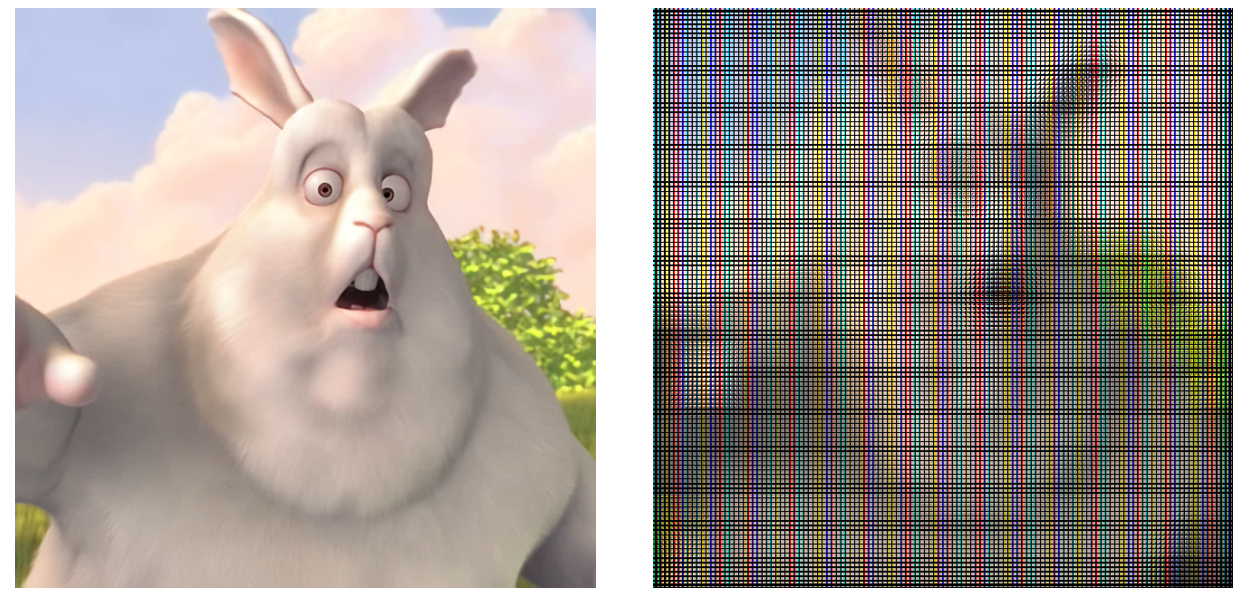
\includegraphics[width=3.5in]{Original_Prefiltered.png}
  \caption{Original Image (left) and Prefiltered Image (right)}
  \label{fig:fr}
\end{figure}

\section{Physical Experiment}

\begin{figure}[ht]
  \centering
  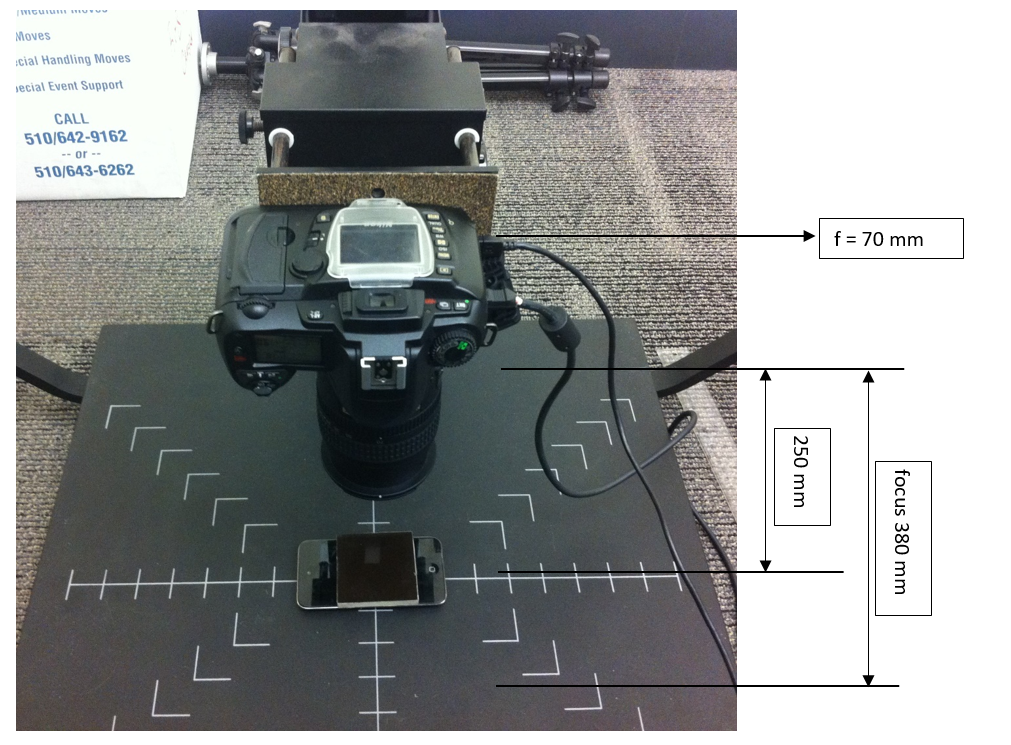
\includegraphics[width=3.5in]{Setup.png}
  \caption{Setup For Physical Experiment}
  \label{fig:ferrari}
\end{figure}

Our physical experiment involves using a camera to simulate a human eye. We set the f-stop of the camera to f/8, and set the f (zoom) to 70 mm. The camera was focused at 380 millimeters and the distance between the camera and the phone was 250 millimeters. Since the camera focuses farther than the object, our setup simulates hyperopia (far-sightedness). Because the pinhole mask blocks a significant portion of light from the iPhone 6, brightness on the phone was increased, and the exposure time was two seconds. To simulate a hyperopic eye, a picture was taken with the original image displayed on the phone. To simulate a corrected eye, a picture was taken with the pinhole mask placed on top of the prefiltered image. 

\begin{figure}[ht]
  \centering
  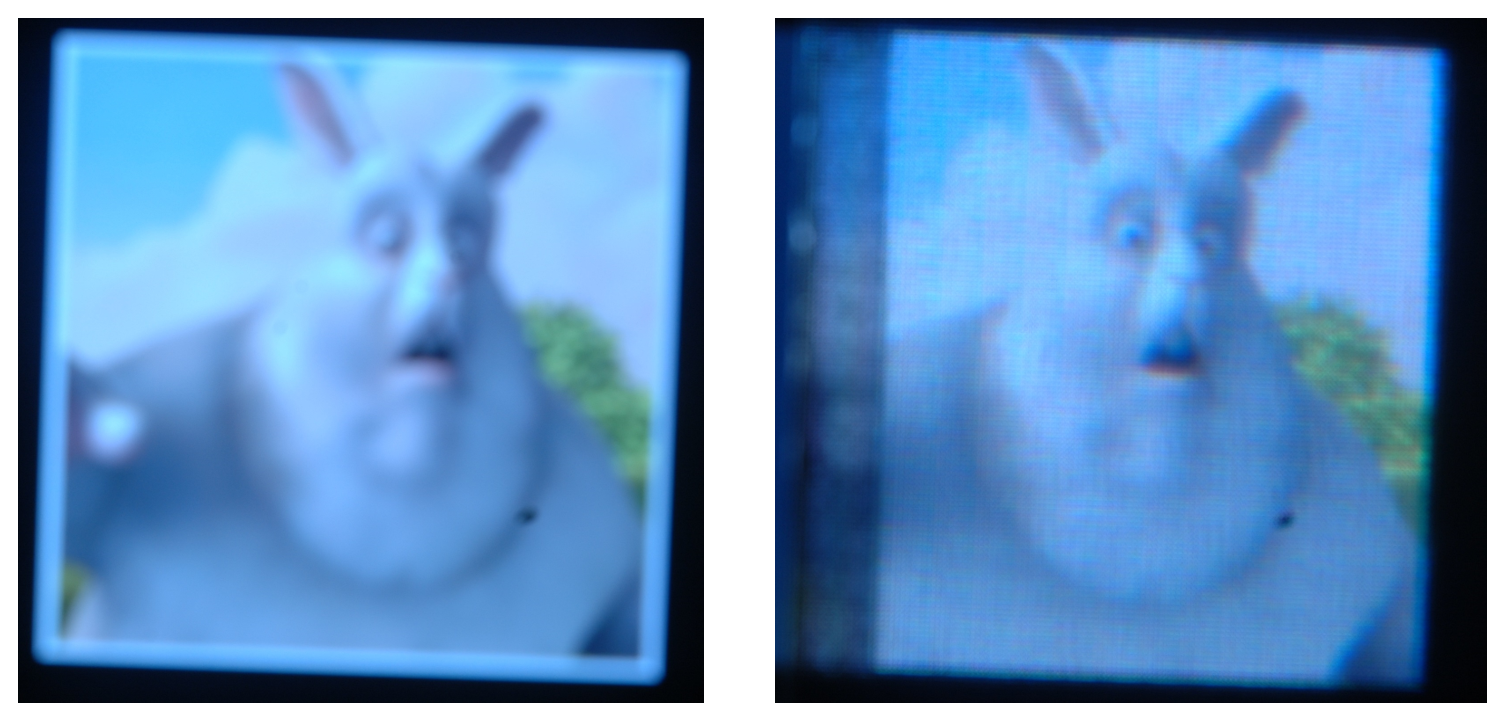
\includegraphics[width=3.5in]{Defocused_Corrected_Image.png}
  \caption{Defocused Image (left) and Corrected Image (right)}
  \label{fig:ferrari}
\end{figure}

The vision correction display yields a significant improvement in the image quality compared to the defocused image. The contrast is higher, and the features of the bunny (eyes, ears, nose, and teeth) are much more noticeable. 

\section{Software Simulation - Ray Optics}

We develop a software simulation to model the effectiveness of the pinhole mask display. There are multiple motivations for the software simulation. One, a software simulation allows experiment parameters, such as focus distance and physical distance to be adjusted more easily. In addition, a pinhole mask display is costly, and the software simulation is used to fine tune the parameters of the pinhole mask, such as depth and pinhole size. Finally, higher order aberrations are difficult to simulate with ordinary lenses, but Zernike polynomials are easy to incorporate into a software simulation.

\begin{figure}[ht]
  \centering
  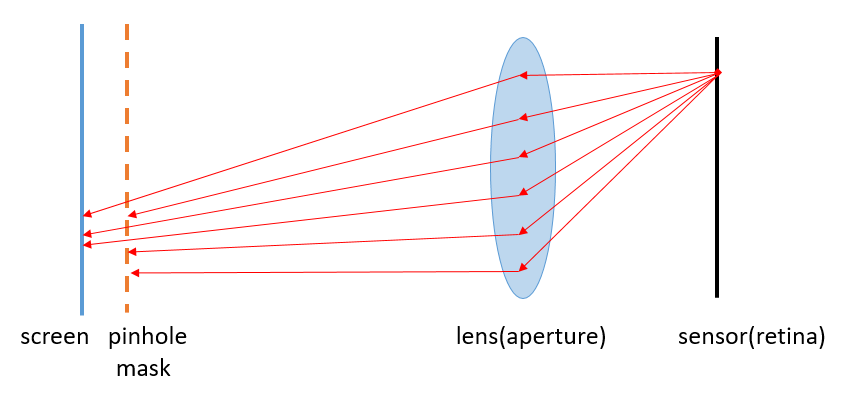
\includegraphics[width=3.3in]{Ray_Simulation.png}
  \caption{Ray Optics Simulation}
  \label{fig:ray_optics}
\end{figure}

One approach we take to simulate the physical experiment is a purely ray optics model. We use a backward ray tracing algorithm, in which light travels from the sensor plane to the display plane. For every pixel on the sensor, the simulation samples multiple points on the aperture (human eye pupil of diameter 6 millimeters). The ray travels straight from the sensor pixel to the aperture point and to the screen. Some of the light rays may get blocked by the pinhole mask or entirely miss the screen. Each screen pixel is composed of a blue, green, and red area, and the color of the ray depends on which position it lands on the screen pixel. Each light ray that reaches the screen contributes to the red, green, or blue intensities of the sensor pixel.

\begin{lstlisting}[frame=single, caption=Pseudocode For Ray Optics Simulation]
int[][][] sensor = new int[sensor_size][sensor_size][3];
// Iterate over sensor pixels
for (int iy = 0; iy < sensor_size; iy++) {
  for (int ix = 0; ix < sensor_size; ix++) {
    int color[3] = {0, 0, 0};
    int hits = 0;
    // Iterate through random aperture points
    for (int i = 0; i < aperture_sample_time; i++) {
      sensor_pos = (ix, iy);
      aperture_pos = (aperture_samples[2*i], aperture_samples[2*i + 1]);
      type,color = getRayColor(sensor_pos, aperture_pos);
      if (value >= 0) {
        hits++;
	color[type] += value;
      }
    }
  }
  sensor[ix][iy] = color * 3 / hits;
}
\end{lstlisting}

In the physical world, each pixel of light travels straight through free space, through the pupil, and hits a point (rod or cone cell) the retina. Each point on the retina may receive light rays from multiple pixels, so the backward ray tracing algorithm does a good job simulating a human eye. 

Another advantage of this approach is that it is simple and easy to parallelize. With OpenCL, a simulation of an image of size $640\times640$ pixels for roughly $1100$ aperture samples runs in less than one minute. This approach can also take into consideration the quantity of light traveling from the screen to the sensor. If the pinhole size is too small, then too many light rays are blocked by the pinhole mask, and the image on the sensor becomes dim due to the lack of light. To fix this issue, we divided the sum of the light rays by the number of hits. \\
\\
One disadvantage of the ray optics model is that it does not take into account wave properties like diffraction and interference. Even though small pinhole sizes are able to focus light more clearly, they also create larger diffraction effects, which this model does not capture. 

\section{Software Simulation - Wave Optics}

We utilize another approach to the software simulation that considers both light traveling as a ray and the diffraction effects of the pinhole. 

\subsection{Fraunhofer Diffraction through Rectangular Aperture}
\noindent We assume that each light ray emits a spherical wavefront that creates a constant electric field on the pinhole. We consider each screen pixel as a point source, and since the depth of the pinhole mask (6 millimeters) is much larger than the size of the screen pixel (78 micrometers) or the pinhole (75 micrometers), the value of the electric field will not vary significantly between the edges of the pinhole and center of the pinhole. The distance between the pinhole plane and the sensor plane is about 27 centimeters, which is much larger than the size of the sensor, so there is not a large variation in the length of different light rays traveling from the mask to the sensor. The pinholes are squares, and we meet the conditions for Fraunhofer diffraction through a rectangular aperture [Lipson, Lipson, and Lipson, 2011]: 
$$\frac{W^2}{L \times \lambda} \ll 1$$
Here, $W$ is the length of the aperture, $L$ is the distance of the sensor from the aperture, and $\lambda$ is the wavelength. $W$ is at most $125$ micrometers, $L$ is roughly $27$ centimeters, and $\lambda$ is about $500$ nanometers. 

\begin{figure}[ht]
  \centering
  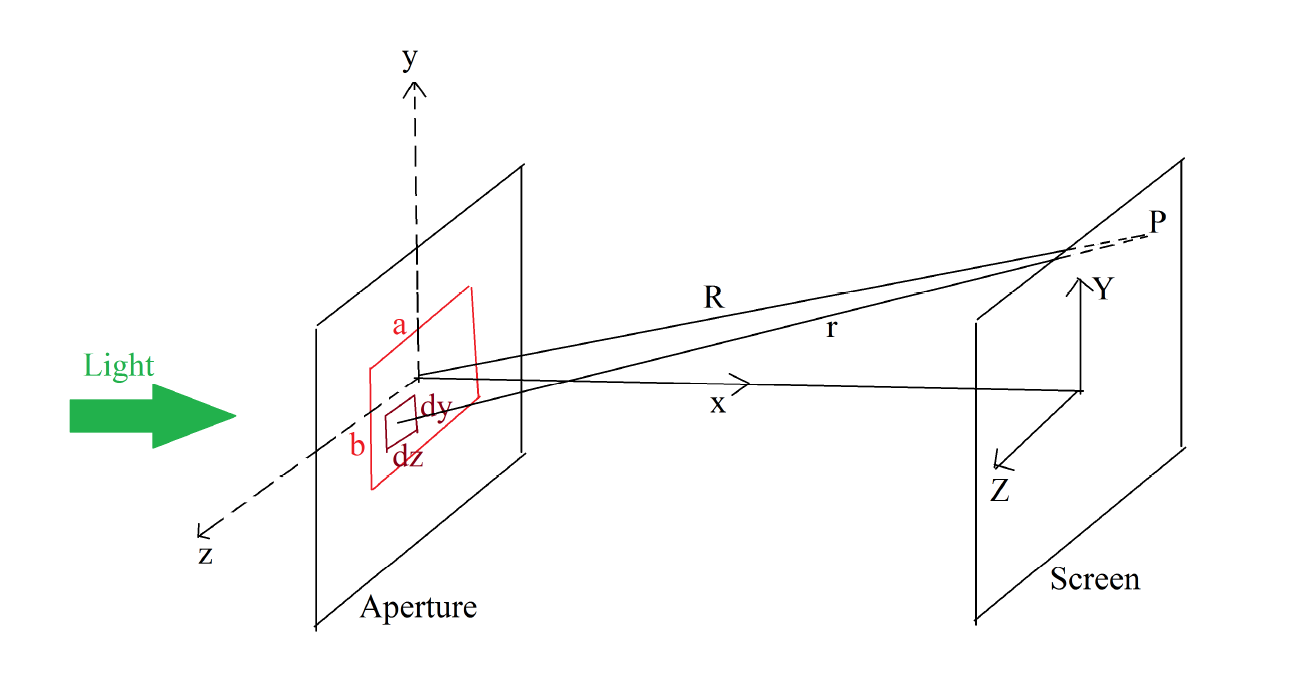
\includegraphics[width=3.5in]{Rectangular_Aperture.png}
  \caption{Fraunhofer Diffraction through Rectangular Aperture Diagram [Rao 2014]}
  \label{fig:ferrari}
\end{figure}

Let $\epsilon_A$ represent the electric field strength per unit area, which is assumed to be constant over the entire aperture (derivation below from Hecht 1987). The electric field contributed by the the small section of the aperture $dzdy$ at point P on the screen is 
$$dE = \left(\frac{\epsilon_A}{R} \right)e^{i(\omega t-kr)}dzdy$$
where $r = [X^2 + (Y-y)^2+(Z-z)^2]^{\frac{1}{2}}$ and $k = \frac{2 \pi}{\lambda}$, the wavenumber. We can use the far field approximation and set $r = R$ for the amplitude term and $r = R[1-(Yy+Zz)^2/{R^2}]$ in the phase term. The total electric field at point $P$ on the screen is \\
$$E = \left(\frac{\epsilon_{A}}{R}\right)e^{i(\omega t-kR)} \int_{-b/2}^{b/2} e^{ikYy/R}dy \int_{-a/2}^{a/2} e^{ikZz/R} dz $$
Solving the integral gives \\
$$E = \left(\frac{ab\epsilon_A}{R}\right) e^{i(\omega t-kR)} sinc\left(\frac{kaZ}{2R}\right)sinc\left(\frac{kbY}{2R}\right) $$ \\
Intensity is equal to the square of the amplitude of the electric field intensity, so \\
$$I(Y,Z) = Re\left[\left(\frac{ab\epsilon_A}{R}\right)e^{i(\omega t - kR)} sinc\left(\frac{kaZ}{2R}\right) sinc\left(\frac{kbY}{2R}\right)\right]^2$$
$$I(Y,Z) = I_0  sinc^2\left(\frac{kaZ}{2R}\right) sinc^2\left(\frac{kbY}{2R}\right)$$
Intensity of light is proportional to two $sinc$ squared functions multiplied in both the $Y$ and $Z$ directions.
% In the future, try to justify your new model.


\subsection{Diffraction through a Lens}
The above diffraction equation creates a very large diffraction pattern on the sensor that leads to far too much loss of contrast. To fix this,we need to consider the effects of the lens and the fact that the display is not placed at the focus distance of 380 millimeters. 

\begin{figure}[ht]
  \centering
  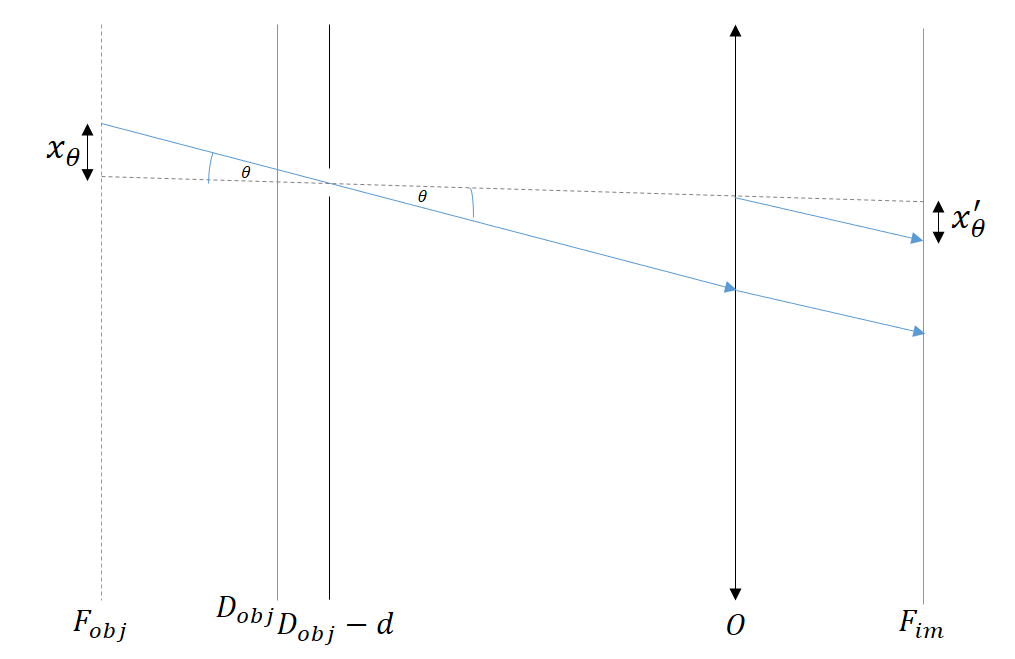
\includegraphics[width=3.5in]{Lens_Diffraction.png}
  \caption{Fraunhofer diffraction through lens. $F_{obj}$ is the focus distance, $D_{obj}$ is the display distance, $d$ is the depth of the pinhole mask, $O$ is the plane of the lens, and $F_{im}$ is equal to position of the sensor at focus.}
  \label{fig:ferrari}
\end{figure}

We know that $$I(Y,Z) = I_0  sinc^2\left(\frac{kaZ}{2R}\right) sinc^2\left(\frac{kbY}{2R}\right)$$
We substitute in $sin(\theta) \sim \frac{Z}{R}$ and $sin(\phi) \sim \frac{Y}{R}$:
$$I(\theta,\phi) = I_0  sinc^2\left(\frac{\pi a sin \theta}{\lambda}\right) sinc^2 \left(\frac{\pi b sin \phi}{\lambda}\right)$$

We want to find the shape of the diffraction pattern as a function of sensor coordinates, $x_{\theta}'$ and $x_{\phi}'$. In other words, we want to determine $I(x_{\theta}', x_{\phi}')$, where $x_{\theta}'$ is the image created by $x_{\theta}$ and $x_{\phi}'$ is the image created by $x_{\phi}$. 

We consider the the angle that light travels through the pinhole, and imagine that the light ray is traced back to the plane at the focus distance. We have: 
$$tan(\theta) = \frac{x_{\theta}}{F_{obj} - D_{obj} + d}$$ 
which gets rearranged to 
$$x_{\theta} = (F_{obj} - D_{obj} + d) tan\theta$$

Then, based on the displacement $x_{\theta}$ on the focus object plane, we can compute the displacement on the sensor $x_{\theta}'$ through the magnification equation. 

$$x_{\theta}' = x_{\theta} \frac{F_{im}}{F_{obj}} =  \frac{F_{im}}{F_{obj}} (F_{obj} - D_{obj} + d) tan\theta $$

Likewise, $$x_{\phi}' = x_{\phi} \frac{F_{im}}{F_{obj}} =  \frac{F_{im}}{F_{obj}} (F_{obj} - D_{obj} + d) tan\phi $$

We want to incorporate the expressions for $x_{\theta}'$ and $x_{\phi}'$ into the original intensity equation. We use the conditions $\theta \ll 1$ (and $\phi \ll 1$) to make the approximations $sin\theta \approx tan\theta \approx \theta$ and $sin\phi \approx tan\phi \approx \phi$. Therefore, 

$$I(\theta, \phi) \approx I_0 sinc^2(\frac{\pi a \theta}{\lambda}) sinc^2(\frac{\pi b \phi}{\lambda})$$

We rearrange $$x_{\theta}' = \frac{F_{im}}{F_{obj}} (F_{obj} - D_{obj} + d) \theta $$ to get $$\theta =  \frac{F_{obj}} {(F_{obj} - D_{obj} + d)F_{im}} x_{\theta}'$$ Likewise,  $$\phi =  \frac{F_{obj}} {(F_{obj} - D_{obj} + d)F_{im}} x_{\phi}'$$ We substitute these results into the intensity equation to get

$$I(x_{\theta}', x_{\phi}') \approx $$ $$I_0 sinc^2 (\frac{\pi a F_{obj} x_{\theta}'}{F_{im}(F_{obj} - D_{obj} + d)\lambda}) sinc^2 (\frac{\pi b F_{obj} x_{\phi}'}{F_{im}(F_{obj} - D_{obj} + d)\lambda})$$

\subsection{Integration of Ray and Wave Optics}

In the integrated ray and wave optics model, ray optics determines the direction of light rays, and wave optics determines the size of the diffraction pattern on the sensor. We continue to do backwards ray tracing on multiple aperture samples, but each ray creates a diffraction pattern on multiple sensor pixels. The combined model is equivalent to blurring the result of the ray optics image by applying a low pass filter, and the blur matrix is determined by the intensities of the diffraction pattern. 

\begin{figure}[ht]
  \centering
  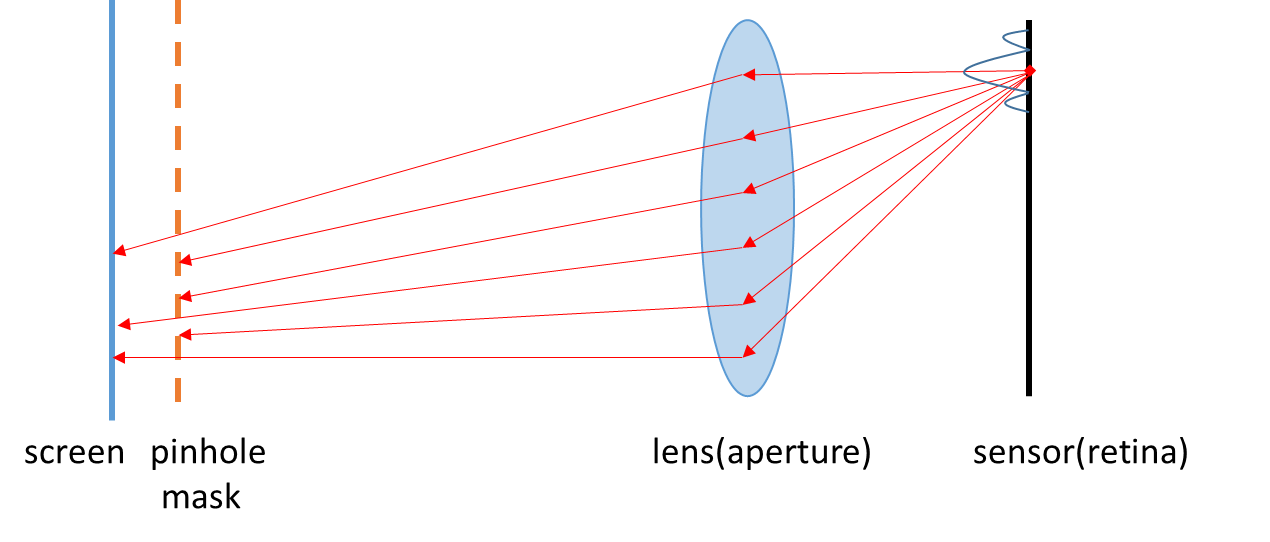
\includegraphics[width=3.5in]{Diffract_Simulation.png}
  \caption{Wave Optics Simulation}
  \label{fig:ferrari}
\end{figure}


\begin{lstlisting} [frame=single, caption=Pseudocode For Wave Optics Simulation]
int[][][] sensor = new int[sensor_size][sensor_size][3];
// Iterate over sensor pixels
for (int iy = 0; iy < sensor_size; iy++) {
  for (int ix = 0; ix < sensor_size; ix++) {
    int color[3] = {0, 0, 0};
    int hits = 0;
    // Iterate through random aperture points
    for (int i = 0; i < aperture_sample_time; i++) {
      sensor_pos = (ix, iy);
      aperture_pos = (aperture_samples[2*i], aperture_samples[2*i + 1]);
      type,color = getRayColor(sensor_pos, aperture_pos);
      if (value >= 0) {
        hits++;
	color[type] += value;
      }
    }
  }
  for (int x = 0; x < diffractMatrix.length; x++) {
    for (int y = 0; y < diffractMatrix.width; y++) {
       sensor[ix + x - diffractMatrix.length / 2][iy + y - diffractMatrix.width/2] += intensity[x][y] * color * 3 / hits;
    }
  }
}
\end{lstlisting}

\section{Results}

We compare the images produced by the physical experiment, ray optics simulation, and wave optics simulation. The parameters for all three cases are the same as those described earlier in the physical experiment section (380 millimeters focus distance, 250 millimeters display distance, 6 millimeters depth of pinhole mask, 6 millimeters diameter of human eye or f/8 stop, and 20 millimeters focal length). In addition, to see how well the ray and wave optics model account for diffraction, we examine the image quality of multiple pinhole sizes.

\subsection{Metrics}

The two metrics used to measure image quality are DRIM (dynamic range imagery) and RMSE (root mean square error).

\subsubsection{DRIM}

Aydin et. al 2008 describes DRIM as a metric that enables comparison of images with different dynamic ranges. The paper describes three measurements of image distortion: loss of visible contrast, amplification of invisible contrast, and reversal of visible contrast. We focus on loss of visible contrast, which occurs when contrast that was visible in the reference image becomes invisible in the test image. The algorithm in the paper applies a loss of visible contrast predictor and then a high-pass or low-pass filter. Here is what the distortion maps look like for the wave optics model for a 75 micrometer pinhole:

\begin{figure}[ht]
  \centering
  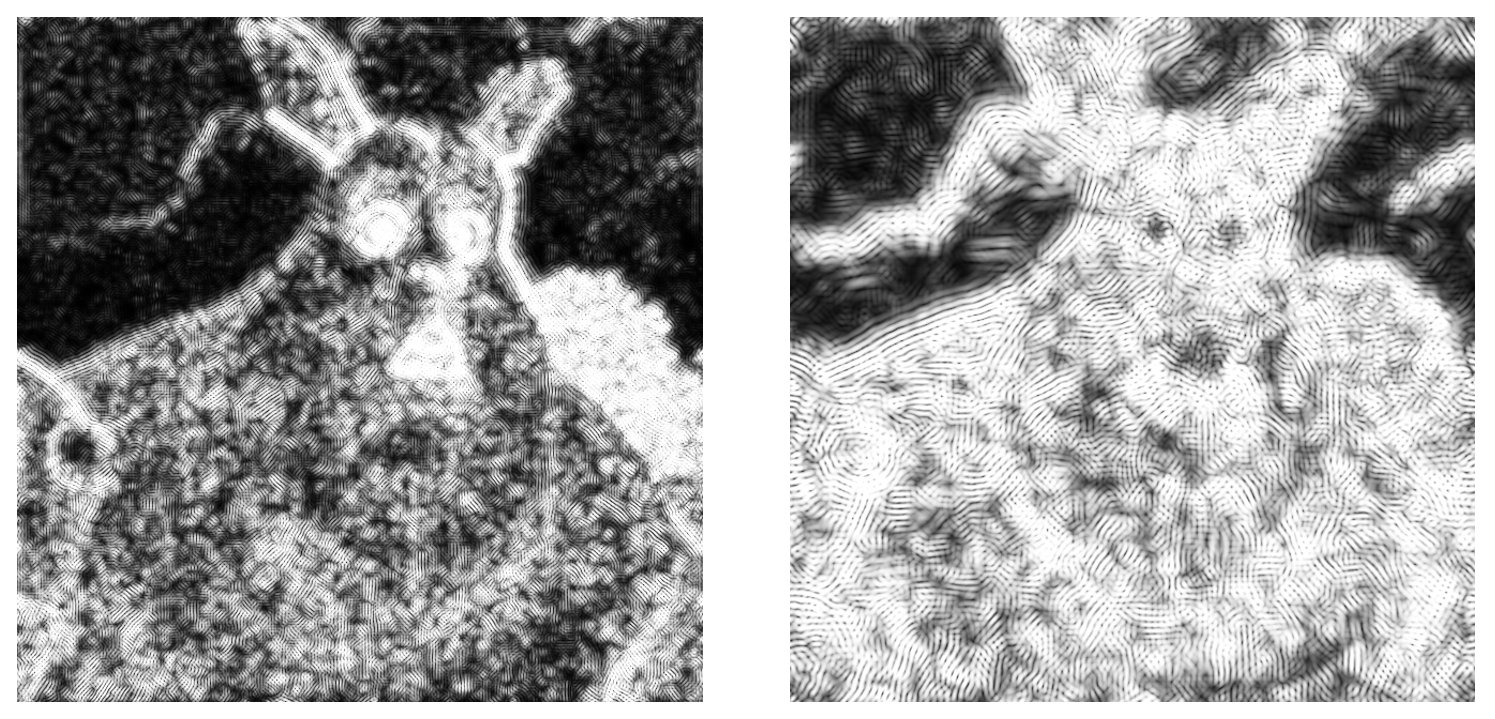
\includegraphics[width=3.5in]{hp_lp_contrast_loss.png}
  \caption{Contrast Loss High Pass (left) and Contrast Loss Low Pass (right)}
  \label{fig:ferrari}
\end{figure}

The bright pixels represent areas of contrast loss. We compute the contrast loss as the pixel sum of the low-pass distortion image plus the pixel sum of the high-pass distortion image divided by two. 

\subsubsection{RMSE}

RMSE is a measurement used to measure how close the pixel values of the test image are to the reference image. $I_r$ in the equation below represents the RGB (red, green, and blue) intensities of the reference image, and $I_t$ represents the RGB intensities of the simulated image.

$$RMSE = \sqrt{ \sum_{y = 0}^{\text{image length}} \sum_{x = 0}^{\text{image width}} \sum_{c \in \{r,g,b\}} (I_r (x,y,c) - I_s(x,y,c))^2}$$

\subsection{Comparison of Ray and Wave Optics}

\begin{figure}[ht]
  \centering
  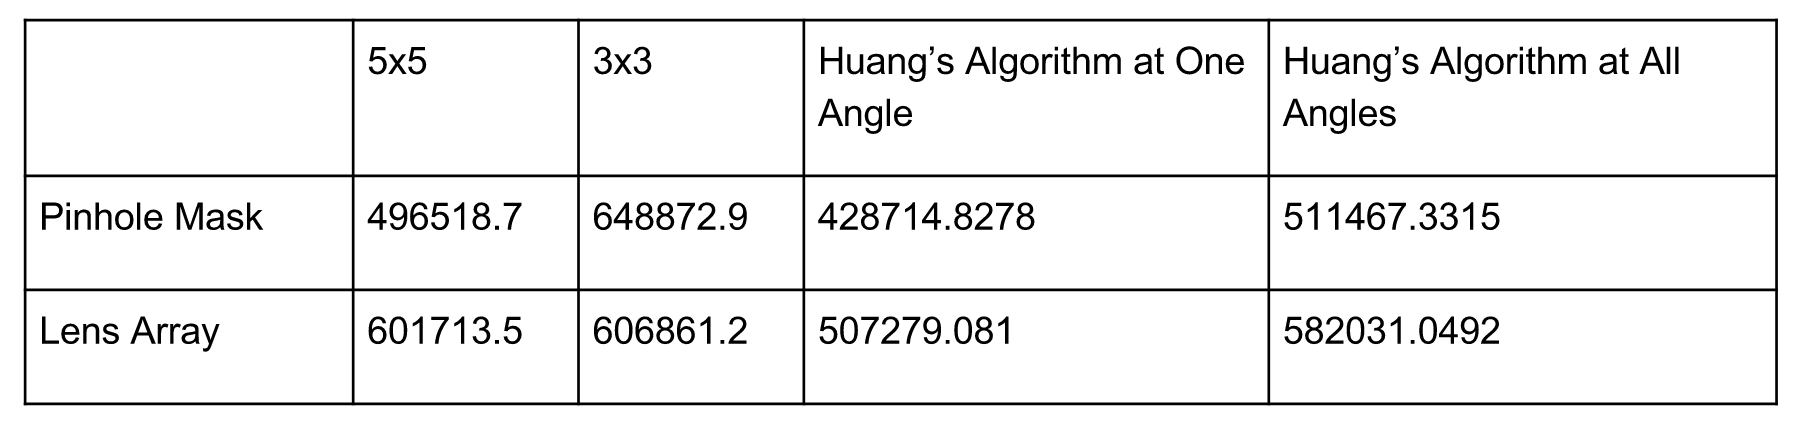
\includegraphics[width=3.5in]{Contrast_Loss.png}
  \caption{DRIM Graph}
  \label{fig:ferrari}
\end{figure}

For the ray optics model, the larger the pinhole size, the worse the contrast. The pinhole size that gives the least loss of contrast is 25 micrometers. A pinhole of size 120 micrometers (contrast loss of about 600,000) generates twice the amount of contrast loss as a pinhole of size 25 micrometers (contrast loss of about 300,000). These results are expected because smaller pinholes focus light, which leads to sharper image contrast. For the combined ray and wave optics model, the contrast loss from different-sized pinholes is roughly the same (between 640,000 and 770,000). We find that the benefits of a small aperture in filtering light are counterbalanced by the larger diffraction pattern that is created. The smallest pinhole sizes create the largest diffraction patterns and therefore have the most severe contrast loss. From 25 micrometers to 105 micrometers, there is a weak trend of improving contrast due to the effects of diffraction outweighing the sharper focus of light through the pinhole. From 105 micrometers to 125 micrometers, there is a weak trend of declining contrast because at that point, the diffraction effects are very minor, and the larger pinhole sizes reduce the depth of field and do not focus the light source well. A pinhole size of 105 microns generates an image with the most contrast.

\begin{figure}[ht]
  \centering
  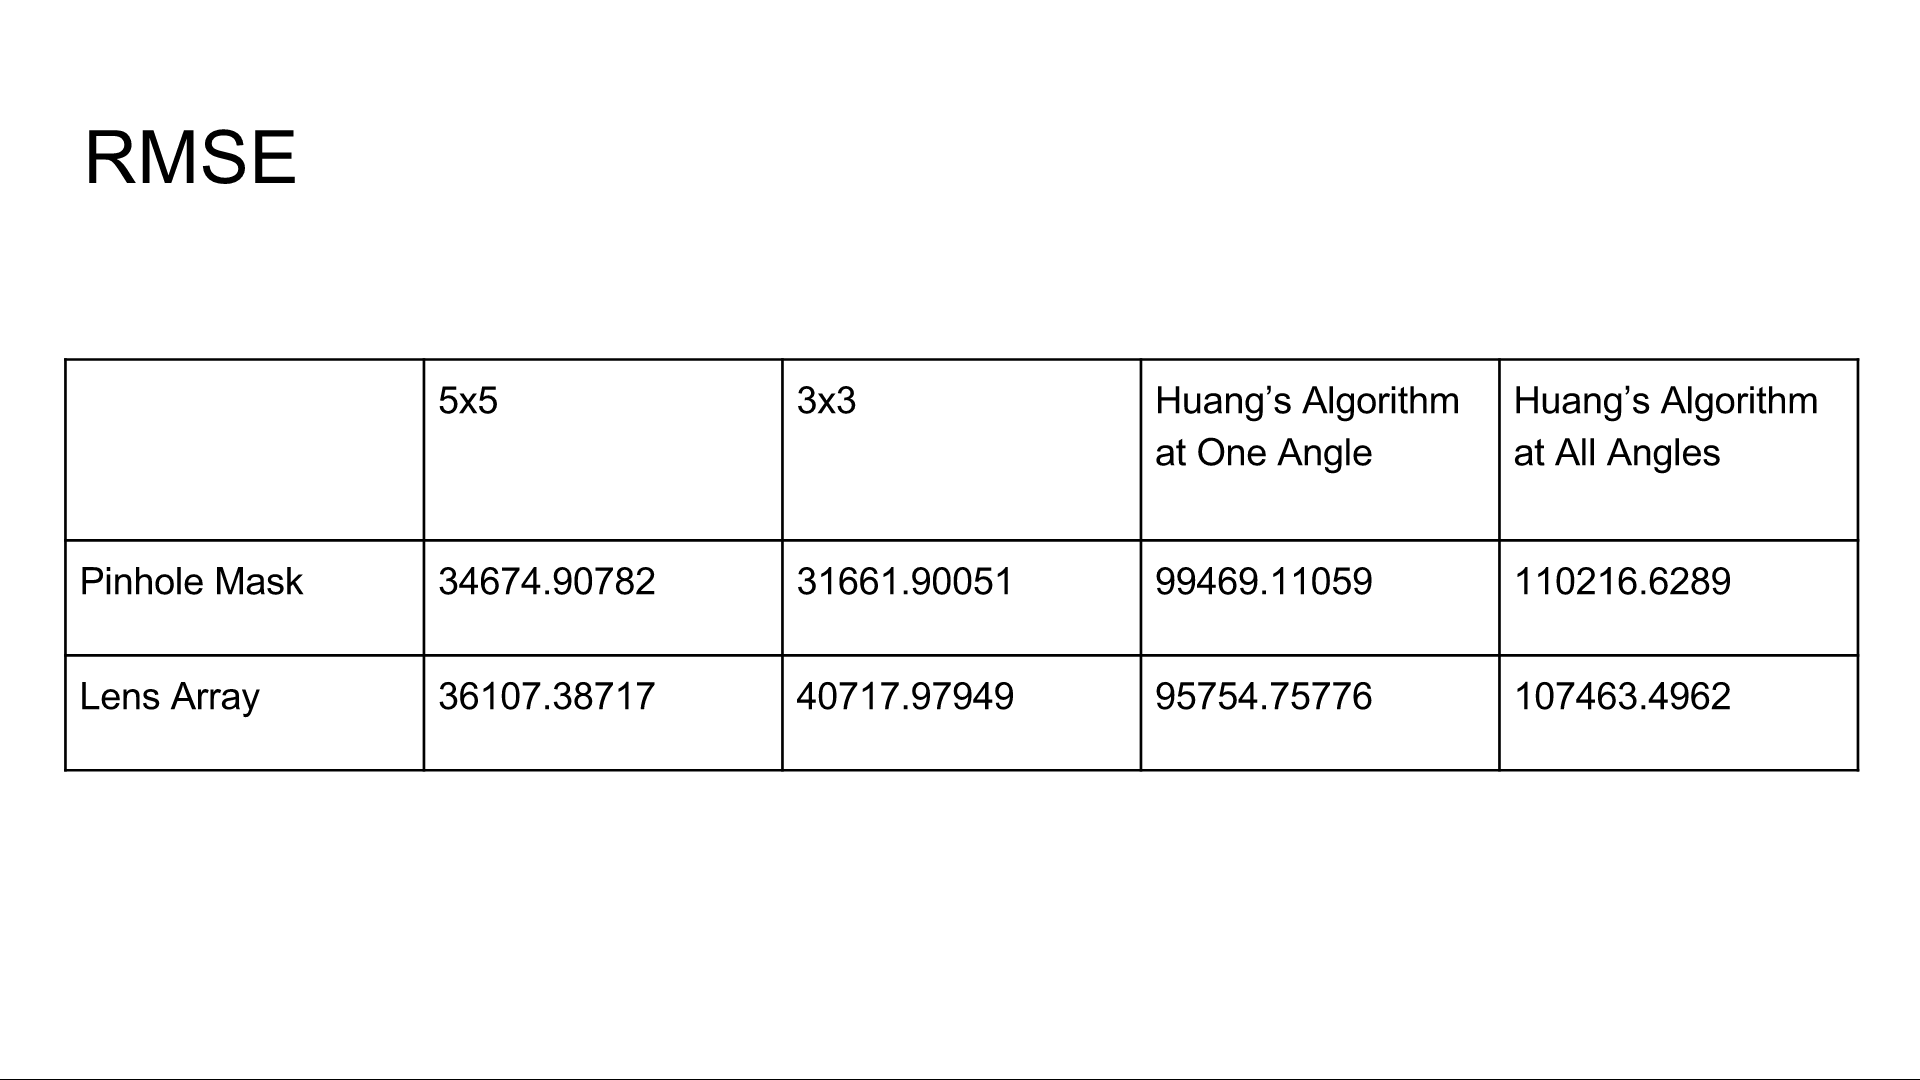
\includegraphics[width=3.5in]{RMSE.png}
  \caption{RMSE Graph}
  \label{fig:ferrari}
\end{figure}

For the RMSE metric, the wave optics model features improvement over the ray optics model, despite the fact that the wave optics model produces a blurred version of the ray optics model. For both models, small pinhole sizes create an amplification of contrast, which leads to a larger RMSE. In addition, since small pinhole sizes allow significantly fewer light rays to reach the screen, there is a greater possibility of having too many rays of one color (red, green, or blue) and getting a noisy image (see figure 14 below). Because blurring reduces this amplification of contrast, larger pinhole sizes have smaller RMSE values for the ray optics model, and the wave optics model consistently produces images with smaller RMSE than the ray optics model. The wave optics model shows a trend of increasing RMSE for pinhole sizes 75 micrometers and above, because at that point, there is no more amplification of contrast, and blurring only causes the modeled image to deviate further from the clean image. Although a smaller RMSE is expected to indicate a image with pixel values close to the original image, it actually has a high chance of indicating more blur. Therefore, RMSE is a poor indicator of contrast and mediocre indicator of image quality. 

\begin{figure}[ht]
  \centering
  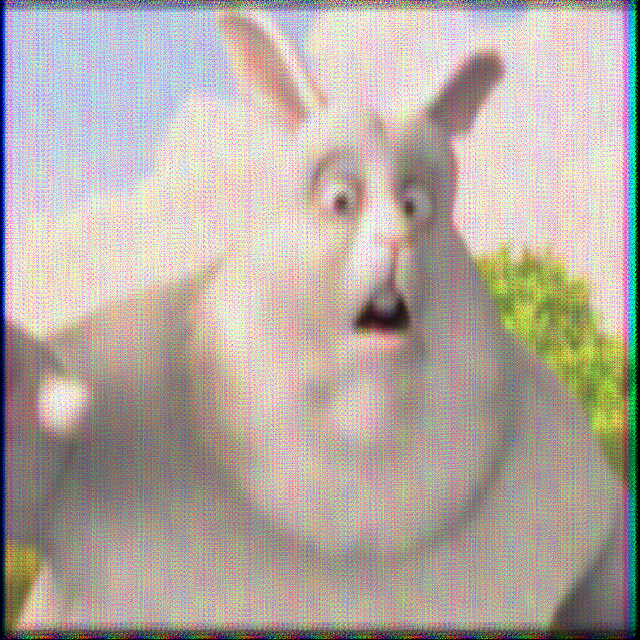
\includegraphics[width=1.5in]{simulationResult_25.png}
  \caption{Ray Optics Simulation for 25 micrometer pinhole mask}
  \label{fig:ferrari}
\end{figure}

\subsection{Comparison of Physical Experiment and Software Simulation}

\begin{figure}[ht]
  \centering
  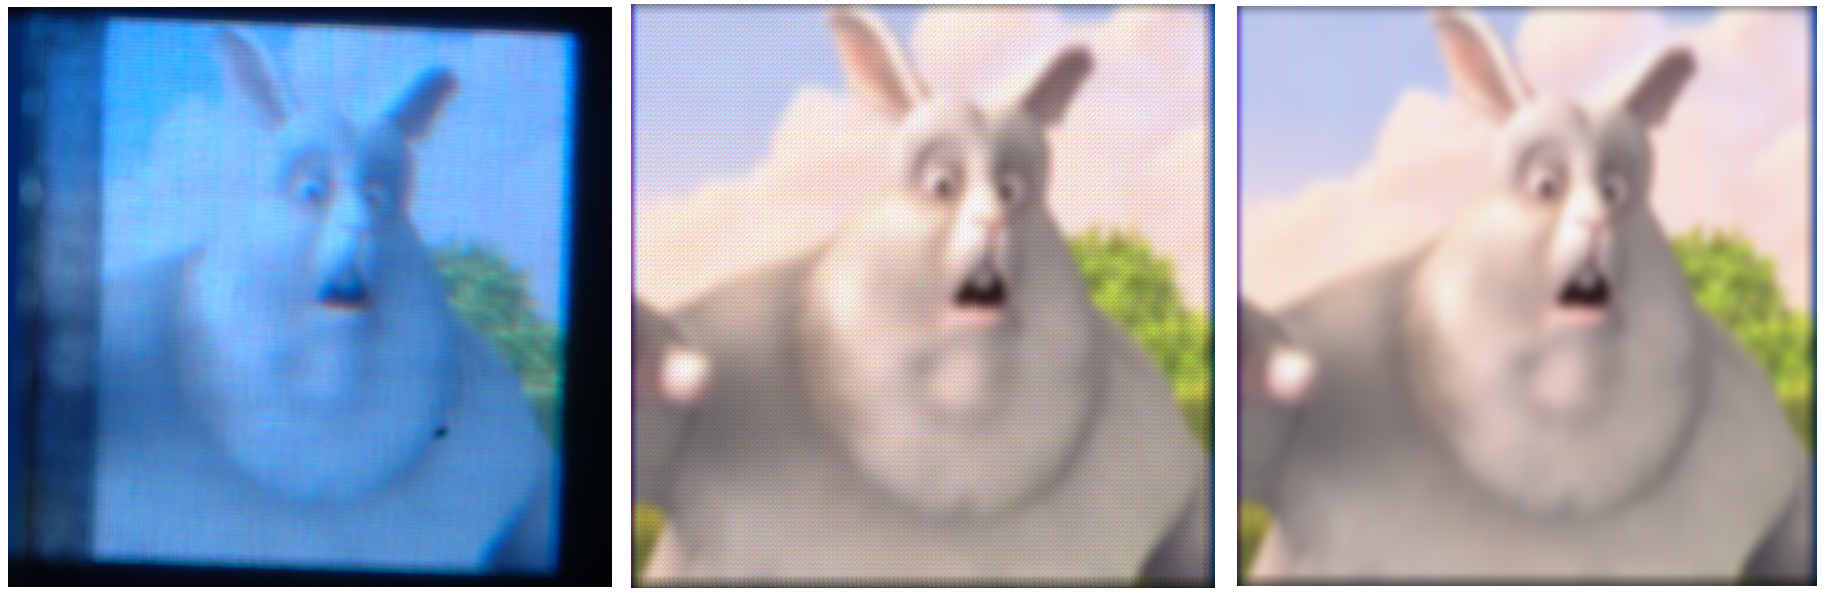
\includegraphics[width=3.5in]{Comparison.png}
  \caption{Comparison of Physical and Software Simulations for 75 micrometer pinhole}
  \label{fig:ferrari}
\end{figure}

We compare the images produced by the physical experiment, ray optics simulation, and wave optics simulation for a 75 micrometer pinhole. The wave optics simulation is slightly more blurred than the ray optics simulation, which is expected. Interestingly enough, the physical simulation generates the clearest image, but the exposure had to be inflated in order for the physical simulation to work. If one looks closely at the physical experiment image and the ray simulation image, one will find that a grid pattern is visible on both the physical experiment image and ray optics image, but is removed from the wave optics image due to diffractional blur. This shows that perhaps the wave optics simulation created a blur pattern that was too large for the 75 micrometer pinhole. 

\section{Conclusion and Future Work}

The physical experiment and the software simulation give mixed results. The prefiltering algorithm combined with the pinhole mask display yields a significant improvement to the defocused image. The ray optics model yields an image that has slightly less contrast than the one in the physical experiment and recommends using the smallest pinhole size to achieve the best contrast as long as RMSE is not too high. The wave optics model gives even more blurred images than the ray optics model and recommends using a larger pinhole size of approximately 105 micrometers to achieve an image with the best constrast. There exists a slight contrast gap between the physical experiment and software simulations that needs to be resolved.

In the future, we will try to find more ways to improve on the ray and wave optics model to look more like the physical experiment. One area to expand on in the wave optics model is to consider the light ray as a Gaussian beam rather than a point source. In addition, we would like to test the ray and wave optics models for astigmatism, another form of lower order aberrations, and higher order aberrations like coma and trefoil. We would also be interested in running physical experiments with pinhole masks for different sizes to confirm the results of the ray and wave optics models. 

% Fix tenses
% Redo charts for 750 and fix sinc function in code

\section*{Acknowledgements}

To Professor Brian Barsky, Michael Chen, Vivek Claver, Alex Jing, Hung Vu, and Yirong Zhen of the vision-correcting display team.

\bibliographystyle{acmsiggraph}
\nocite{*}
\bibliography{template}

\end{document}
